\section{Čtvrtý týden}

\subsection{Konvexní funkce}
Nechť $f : D \subseteq \R^n \rightarrow \R$ a $C \subseteq D$ je neprázdná konvexní množina. \\
Řekněme, že $f$ je
\begin{enumerate}[(a)]
    \item konvexní na $C$, jestliže pro každé $x, y \in C$ a každé $\lambda \in [0,1]$ je 
    \[
        f(\lambda x + (1-\lambda) y) \leq \lambda f(x) + (1-\lambda)f(y).
    \]
    \item ryze konvexní na $C$, jestliže pro každé dva různé body $x, y \in C$ a $\lambda \in (0,1)$ je
    \[
        f(\lambda x + (1-\lambda) y) < \lambda f(x) + (1-\lambda)f(y).
    \]
    \item konkávní (resp. ryze konkávní) na $C$, jestliže $(-f)$ je konvexní (resp. ryze konvexní) na $C$.
\end{enumerate}

\begin{multicols}{2}
    \begin{tikzpicture}[scale=2]
        \draw[->] (-2,0) -- (2,0);
        \draw[->] (0,-0.5) -- (0,3);
        
        \draw[thick, blue, domain=-1.5:1.5, smooth] plot (\x, {(\x)^2 + 0.5});
        
        \node at (1.2,2.3) [below right]{\small \textcolor{blue}{$f(x)$}};
    
        \draw[black!40!yellow, thick] (-1, 1.5) -- (0.5, 0.75);
    
        \draw[black!40!green, dashed] (-1,1.5) -- (-1, 0) node[below]{\small $x$};
        \fill[black!40!green] (-1, 1.5) circle(1pt) node[left]{\small $(x, f(x))$};
    
        \draw[black!40!red, dashed] (0.5,0.75) -- (0.5, 0) node[below]{\small $y$};
        \fill[black!40!red] (0.5, 0.75) circle(1pt) node[right]{\small $(y, f(y))$};
    
        \draw[yellow!40!red, dashed] (-0.25, 1/16 + 0.5) -- (-0.25, -0.05) node[below]{\small $C$};
        \fill[yellow!40!red] (-0.25, 1/16 + 0.5) circle(1pt) node[below left]{\small $B$};
        % \draw[yellow!40!red, <-] (-0.25 - 0.1, 1/16 + 0.5 + 0.03) -- (-0.75, 0.7) node[left]{\small $B$};
    
        \draw[yellow!40!red, dashed] (-0.25, 1/16 + 0.5) -- (-0.25, 1/16 + 1 + 1/16);
        \fill[yellow!40!red] (-0.25, 1/16 + 1 + 1/16) circle(1pt) node[below left]{\small $A$};
        % \draw[yellow!40!red, <-] (-0.25, 1/16 + 1 + 1/16 + 0.05) -- (-0.75, 1.7) node[left]{\small $A$};
    
    \end{tikzpicture}

\columnbreak

    \textcolor{yellow!40!red}{$A$} $= (\lambda x + (1-\lambda)y, \lambda f(x) + (1-\lambda)f(y))$\\
    \textcolor{yellow!40!red}{$B$} $= (\lambda x + (1-\lambda)y, f(\lambda x + (1-\lambda)y))$\\
    \textcolor{yellow!40!red}{$C$} $= \lambda x + (1-\lambda)y$

    Pozorování: \textcolor{black!40!yellow}{úsečka} vždy leží nad \textcolor{blue}{funkcí}.
\end{multicols}

\subsection{Příklad konvexní funkce}
Je afinní zobrazení $f : \R^n \rightarrow \R^n$ (tj. $f(x) = \langle x,a \rangle + b, b\in \R$) konvexní?

Důkaz.\\
Ať  $x, y \in \R^n, \lambda \in [0,1]$.
\begin{align*}
    f(\lambda x + (1-\lambda) y) &= \langle \lambda x + (1-\lambda) y, a\rangle + b\\
    &= \lambda \langle x, a\rangle + (1-\lambda) \langle y, a\rangle + \lambda b + (1-\lambda)b\\
    &= \lambda f(x) + (1-\lambda) f(y) \implies f \text{ je konvexní i konkávní.} \qed
\end{align*}

\subsection{Příklad konvexní funkce}
Je funkce $f(x) = \| x\|$ konvexní?

Důkaz.\\
Ať Ať  $x, y \in \R^n, \lambda \in [0,1]$.

\[
    f(\lambda x + (1-\lambda) y) = \| \lambda x + (1-\lambda)y\| \stackrel{\text{odhad}}{\leq} \| \lambda x\| + 
    \| (1-\lambda) y\| = \lambda \| x\| + (1-\lambda) \| y\|
\]
\[
    = \lambda f(x) + (1-\lambda) f(y) \implies f \text{ je konvexní.} \qed
\]

\subsection{Dolní úrovňová množina}
Dolní úrovňování množina funkce $f : D \subseteq \R^n \rightarrow \R^n$ hladiny $\alpha \in \R$ je množina
\[
    \lev_{\leq} (f; \alpha) := \bc{x \in D \mid f(x) \leq \alpha}.
\]
Je-li $f$ konvexní na $C \subseteq \R^n$, pak $\lev_{\leq} (\restr{f}{C}; \alpha)$ je konvexní pro $\forall \alpha \in \R$.


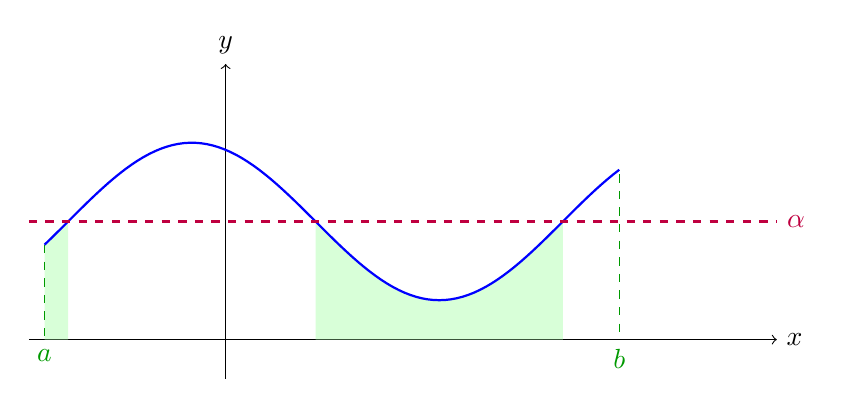
\begin{tikzpicture}[domain=-0.3:7, samples=100]
    \draw[->] (-2.5,0) -- (7,0) node[right] {$x$};
    \draw[->] (0,-0.5) -- (0,3.5) node[above] {$y$};

    % Segment I: x in [-2.3, -2]
    \fill[green!30, opacity=0.5]
    plot[domain=-2.3:-2, samples=50] (\x, {sin((\x+2) r)+1.5})
    -- (-2,0) -- (-2.3,0) -- cycle;
    
    % % Segment II: x in [-2, pi-2]
    % \fill[green!30, opacity=0.5]
    % (-2,1.5) -- ({pi-2},1.5) -- ({pi-2},0) -- (-2,0) -- cycle;
    
    % Segment III: x in [pi-2, 2*pi-2]
    \fill[green!30, opacity=0.5]
    plot[domain={pi-2}:{2*pi-2}, samples=50] (\x, {sin((\x+2) r)+1.5})
    -- ({2*pi-2},0) -- ({pi-2},0) -- cycle;
    
    % % Segment IV: x in [2*pi-2, 5]
    % \fill[green!30, opacity=0.5]
    % ({2*pi-2},1.5) -- (5,1.5) -- (5,0) -- ({2*pi-2},0) -- cycle;
    
    \draw[blue, thick] plot ({\x-2}, {sin(\x r) + 1.5});

    \draw[purple, thick, dashed] (-2.5, 1.5) -- (7, 1.5) node[right]{$\alpha$};

    \draw[black!40!green, dashed] (-2.3, 1.2) -- (-2.3, 0) node[below]{$a$};
    \draw[black!40!green, dashed] (5, 2.1) -- (5, 0) node[below]{$b$};
\end{tikzpicture}

Důkaz.

Ať $x, y \in \lev_{\leq}(\restr{f}{C}; \alpha), \lambda \in [0,1]$.\\
Cíl: $\lambda x + (1-y)\lambda \stackrel{?}{\in} \lev_{\leq} (\restr{f}{C}; y)$.
\[
    f(\lambda x + (1-\lambda)y) \leq \lambda f(x) + (1-\lambda) f(y) \leq \lambda \alpha + (1-\lambda) \alpha = \alpha. \qed
\]

Poznámka.

Opačná implikace neplatí. Tedy pomocí dolní úrovňové množiny \textbf{nelze} určit, jestli původní funkce je konvexní.

Například $f = x^3$ není konvexní funkce na intervalu $x = [-2, 2]$, ale když zvolíme $\alpha = 8$, tak dolní úrovňová 
množina bude konvexní. % TODO nákres

\subsection{Použití dolní úrovňové množiny}
Je množina $M = \bc{x \in \R^2 \mid \| x\| \leq 1, \left\langle x, 
\begin{pmatrix}
    2 \\
    1
\end{pmatrix}
\right\rangle \leq 1}$ konvexní?

Důkaz.

Rozdělme si množinu $M$ na dvě podmnožiny $M_1$ a $M_2$, kde:

$M_1 = \bc{x \in \R^2 \mid \| x\| \leq 1} = \lev_{\leq} (\| x\|, 1) \rightarrow$ konvexní, protože norma je konvexní funkce.

$M_2 = \bc{x \in \R^2 \mid \left\langle x, 
\begin{pmatrix}
    2 \\
    1
\end{pmatrix}
\right\rangle \leq 1} = \lev_{\leq} \left(\left\langle x, 
\begin{pmatrix}
    2 \\
    1
\end{pmatrix}
\right\rangle, 1\right) \rightarrow$ konvexní, protože skalární součin je konvexní.

To nám ale dává průnik dvou konvexních množin, tedy $M = M_1 \cap M_2$ je také konvexní. $\qed$

% TODO nákres

\subsection{Součet a součin zachovávají konvexitu}\label{ssKonv}
Mějme funkce $f, g$, které jsou konvexní na $C$, $\alpha \geq 0$. Pak:
\begin{enumerate}[(a)]
    \item $f+g$ je konvexní na $C$
    \item $\alpha f$ je konvexní na $C$
\end{enumerate}

Důkaz.

(a) Ať $\lambda \in [0,1], x, y \in C$.
\[
    (f+g)(\lambda x + (1-\lambda)y) = \underbrace{f(\lambda x + (1-\lambda)y)}_{\leq \lambda f(x) + (1-\lambda)f(y)} + 
    \underbrace{g(\lambda x + (1-\lambda)y)}_{\leq \lambda g(x) + (1-\lambda)g(y)}
\]
\[
    \leq \lambda f(x) + (1-\lambda)f(y) + \lambda g(x) + (1-\lambda)g(y) = \lambda (f+g)(x) + (1-\lambda)(f+g)(y). \qed
\]

(b) Ať $\lambda \in [0,1], x, y \in C, \alpha \geq 0$. % TODO dodělat důkaz


\subsection{Příklad ověření konvexity}
Je funkce $f(x) = e^x - 3 \ln x + 2x$ konvexní?

Rozeberme si jednotlivé části funkce.
\begin{itemize}
    \item $e^x$ $\dots$ exponenciála je z grafu očividně konvexní.
    \item $-3 \ln x$ $\dots$ logaritmus je konkávní, ale díky \enquote{$\minus$} se celý výraz stane konvexní. Násobení konstatou 
    konvexitu neovlivní, viz důkaz \hyperref[ssKonv]{(b)}.
    \item $2x$ $\dots$ lineární funkce je konvexní.
\end{itemize}
Protože všechny komponenty funkce $f$ jsou konvexní, pak je i funkce $f$ nutně konvexní.